\documentclass[11pt]{article}

% --- Page layout ---
\usepackage[a4paper,margin=2cm]{geometry}

% --- Typography and section formatting ---
\usepackage{titlesec}
\titleformat{\section}{\normalfont\Large\bfseries}{}{0pt}{}
\titleformat{\subsection}{\normalfont\large\bfseries}{}{0pt}{}
\usepackage{parskip}

% --- Figures and tables ---
\usepackage{graphicx}
\usepackage{float}
\usepackage{booktabs}
\usepackage{caption}
\usepackage{subcaption}
\captionsetup[figure]{justification=centering}
\usepackage{url}
\usepackage{booktabs}
\usepackage{array}
\newcolumntype{M}[1]{>{\centering\arraybackslash}m{#1}}
\usepackage{amsmath}

% --- Document starts here ---
\begin{document}
	
	\begin{center}
		\LARGE\textbf{Bayesian Spatial Risk Modelling of Suicide Mortality in South Korea Using the ICAR Model}
	\end{center}
	
	\section*{Introduction}
	
	South Korea consistently reports one of the highest suicide rates among developed nations, with 24 to 28 deaths per 100,000 people in recent years—nearly twice the OECD average of 11 (Kim, 2024). Although rates declined modestly in the mid-2010s following national prevention efforts, they have since resurged, reaching 28.3 per 100,000 in 2024—the highest level in over a decade (YNA, 2025). This persistent trend positions South Korea as a global outlier and underscores the urgent need to investigate its underlying risk factors. A large body of research shows that suicide rates are shaped by a mix of socioeconomic, demographic, cultural, and psychological factors. Classical theories dating back to Durkheim (1951) emphasise the protective role of social integration, while economic hardship and mental illness remain key drivers of suicide. In South Korea, national crises such as the late 1990s Asian financial crash have been linked to suicide spikes, primarily through rising unemployment and social dislocation (Chang, 2009).
	
	Among the many determinants examined, social isolation have been identified as a major risk factor. Individuals living alone or lacking family support are more vulnerable due to loneliness and reduced integration. In South Korea, areas with more single-person households or divorced residents tend to have higher suicide rates (Jang, 2022), reflecting the link between weaker social ties and suicide risk. Psychological stress is another significant factor. South Korea reports high levels of perceived stress, which is associated with depression and suicide ideation (Oh, 2020). The indicator "stress awareness"—the proportion of people experiencing significant stress—has been linked to higher suicide rates at the regional level (Jang, 2022). Unemployment is a well-documented driver. Job loss can trigger financial strain, identity loss, and psychological distress. Park and Lester (2006) identified unemployment as a key contributor to South Korea's suicide rate, particularly where social safety nets are weak. Lastly, unmet medical needs reflect gaps in healthcare access, including mental health services. Though 90\% of people who die by suicide have a diagnosable condition, only about 15\% ever receive treatment. Kim (2022) finds that regions with higher unmet medical needs tend to experience higher suicide mortality.
	
	Given the spatially patterned nature of suicide, advanced statistical methods are needed to separate risk factors from geographic influences. We use a Bayesian Intrinsic Conditional Auto-Regressive (ICAR) model, which incorporates information from adjacent regions to produce more stable small-area risk estimates. Our analysis includes four key covariates discussed above, alongside spatial random effects to assess their contribution to geographic variation. This modelling framework accounts for unobserved spatial influences and estimates exceedance probabilites to identify municipalities where suicide risk surpasses a defined threshold. Our key outputs will provide localised insights into suicide risk and guide targeted public health interventions and efficient resource allocation across South Korea.

	\section*{1. Data and Methods}
	
	\subsection*{1.1 Study Area and Spatial Units}
	
	The study area encompasses all 229 municipalities in South Korea, including cities (\textit{shi}), counties (\textit{kun}), and districts (\textit{ku}), collectively referred to as \textit{shikunku}-level administrative units. This spatial resolution was selected as it represents the most granular level for which all variables were consistently available, and aligns with the administrative scale at which suicide prevention policies are typically formulated and implemented. Spatial boundaries were based on official 2022 shapefiles, to which all statistical datasets were harmonised by resolving naming inconsistencies, aggregating sub-municipal divisions, and correcting backdated administrative updates. To ensure spatial contiguity for modelling, disconnected island polygons were linked to the mainland subgraph via nearest-neighbour centroids, restoring connectivity in the spatial adjacency structure.
	
	\subsection*{1.2 Target and Predictor Variables}
	
	The primary outcome variable is the number of suicide deaths in 2022 at the municipality (\textit{shikunku}) level, estimated by multiplying the age-standardised suicide rate (per 100,000 people) by the mid-year population for each municipality. Suicide rates were obtained from Statistics Korea's Cause of Death Statistics, and population estimates from the 2022 Future Population Projections. This indirect approach was required due to the absence of disaggregated suicide counts at this spatial resolution.
	
	Four predictor variables were selected based on their relevance in the literature: the proportion of single-person households, stress awareness rate, unemployment rate, and unmet medical needs rate. All predictors reflect conditions in 2022 and were sourced from national databases including the Population and Housing Census, the Community Health Survey, and the Local Employment Statistics.
	
	\begin{table}[H]
		\centering
		\caption{Summary of Datasets Used in the Analysis}
		\renewcommand{\arraystretch}{1.4}
		\resizebox{\textwidth}{!}{%
			\begin{tabular}{M{4.5cm} M{4.5cm} M{3.5cm} M{5cm} M{1.2cm}}
				\toprule
				\textbf{Variable} & \textbf{Dataset} & \textbf{Usage} & \textbf{Source} & \textbf{Year} \\
				\midrule
				\textbf{Suicide Rate} & Cause of Death Statistics & Target variable & Statistics Korea (Population Trends Division) & 2022 \\
				\textbf{Single-Person Household Ratio} & Population and Housing Census & Predictor variable & Statistics Korea (Population and Housing Census Division) & 2022 \\
				\textbf{Stress Awareness Rate} & Community Health Survey & Predictor variable & Korea Disease Control and Prevention Agency (KDCA) & 2022 \\
				\textbf{Unemployment Rate} & Local Employment Statistics & Predictor variable & Statistics Korea (Employment Statistics Division) & 2022 \\
				\textbf{Unmet Medical Needs Rate} & Community Health Survey & Predictor variable & Korea Disease Control and Prevention Agency (KDCA) & 2022 \\
				\textbf{Estimated Population} & Future Population Projections & Standardisation / Denominator & Statistics Korea (Regional Statistics Planning Division) & 2022 \\
				\textbf{Municipality Boundaries} & Municipality Shapefiles & Spatial analysis & Statistical Geographic Information System (SGIS) & 2022 \\
				\textbf{Province Boundaries} & Province Shapefiles & Mapping / Labelling & Statistical Geographic Information System (SGIS) & 2022 \\
				\bottomrule
			\end{tabular}
		}
		\label{tab:datasets}
	\end{table}
	
	\begin{figure}[H]
		\centering
		\caption{Suicide Rates Across South Korean Municipalities}
		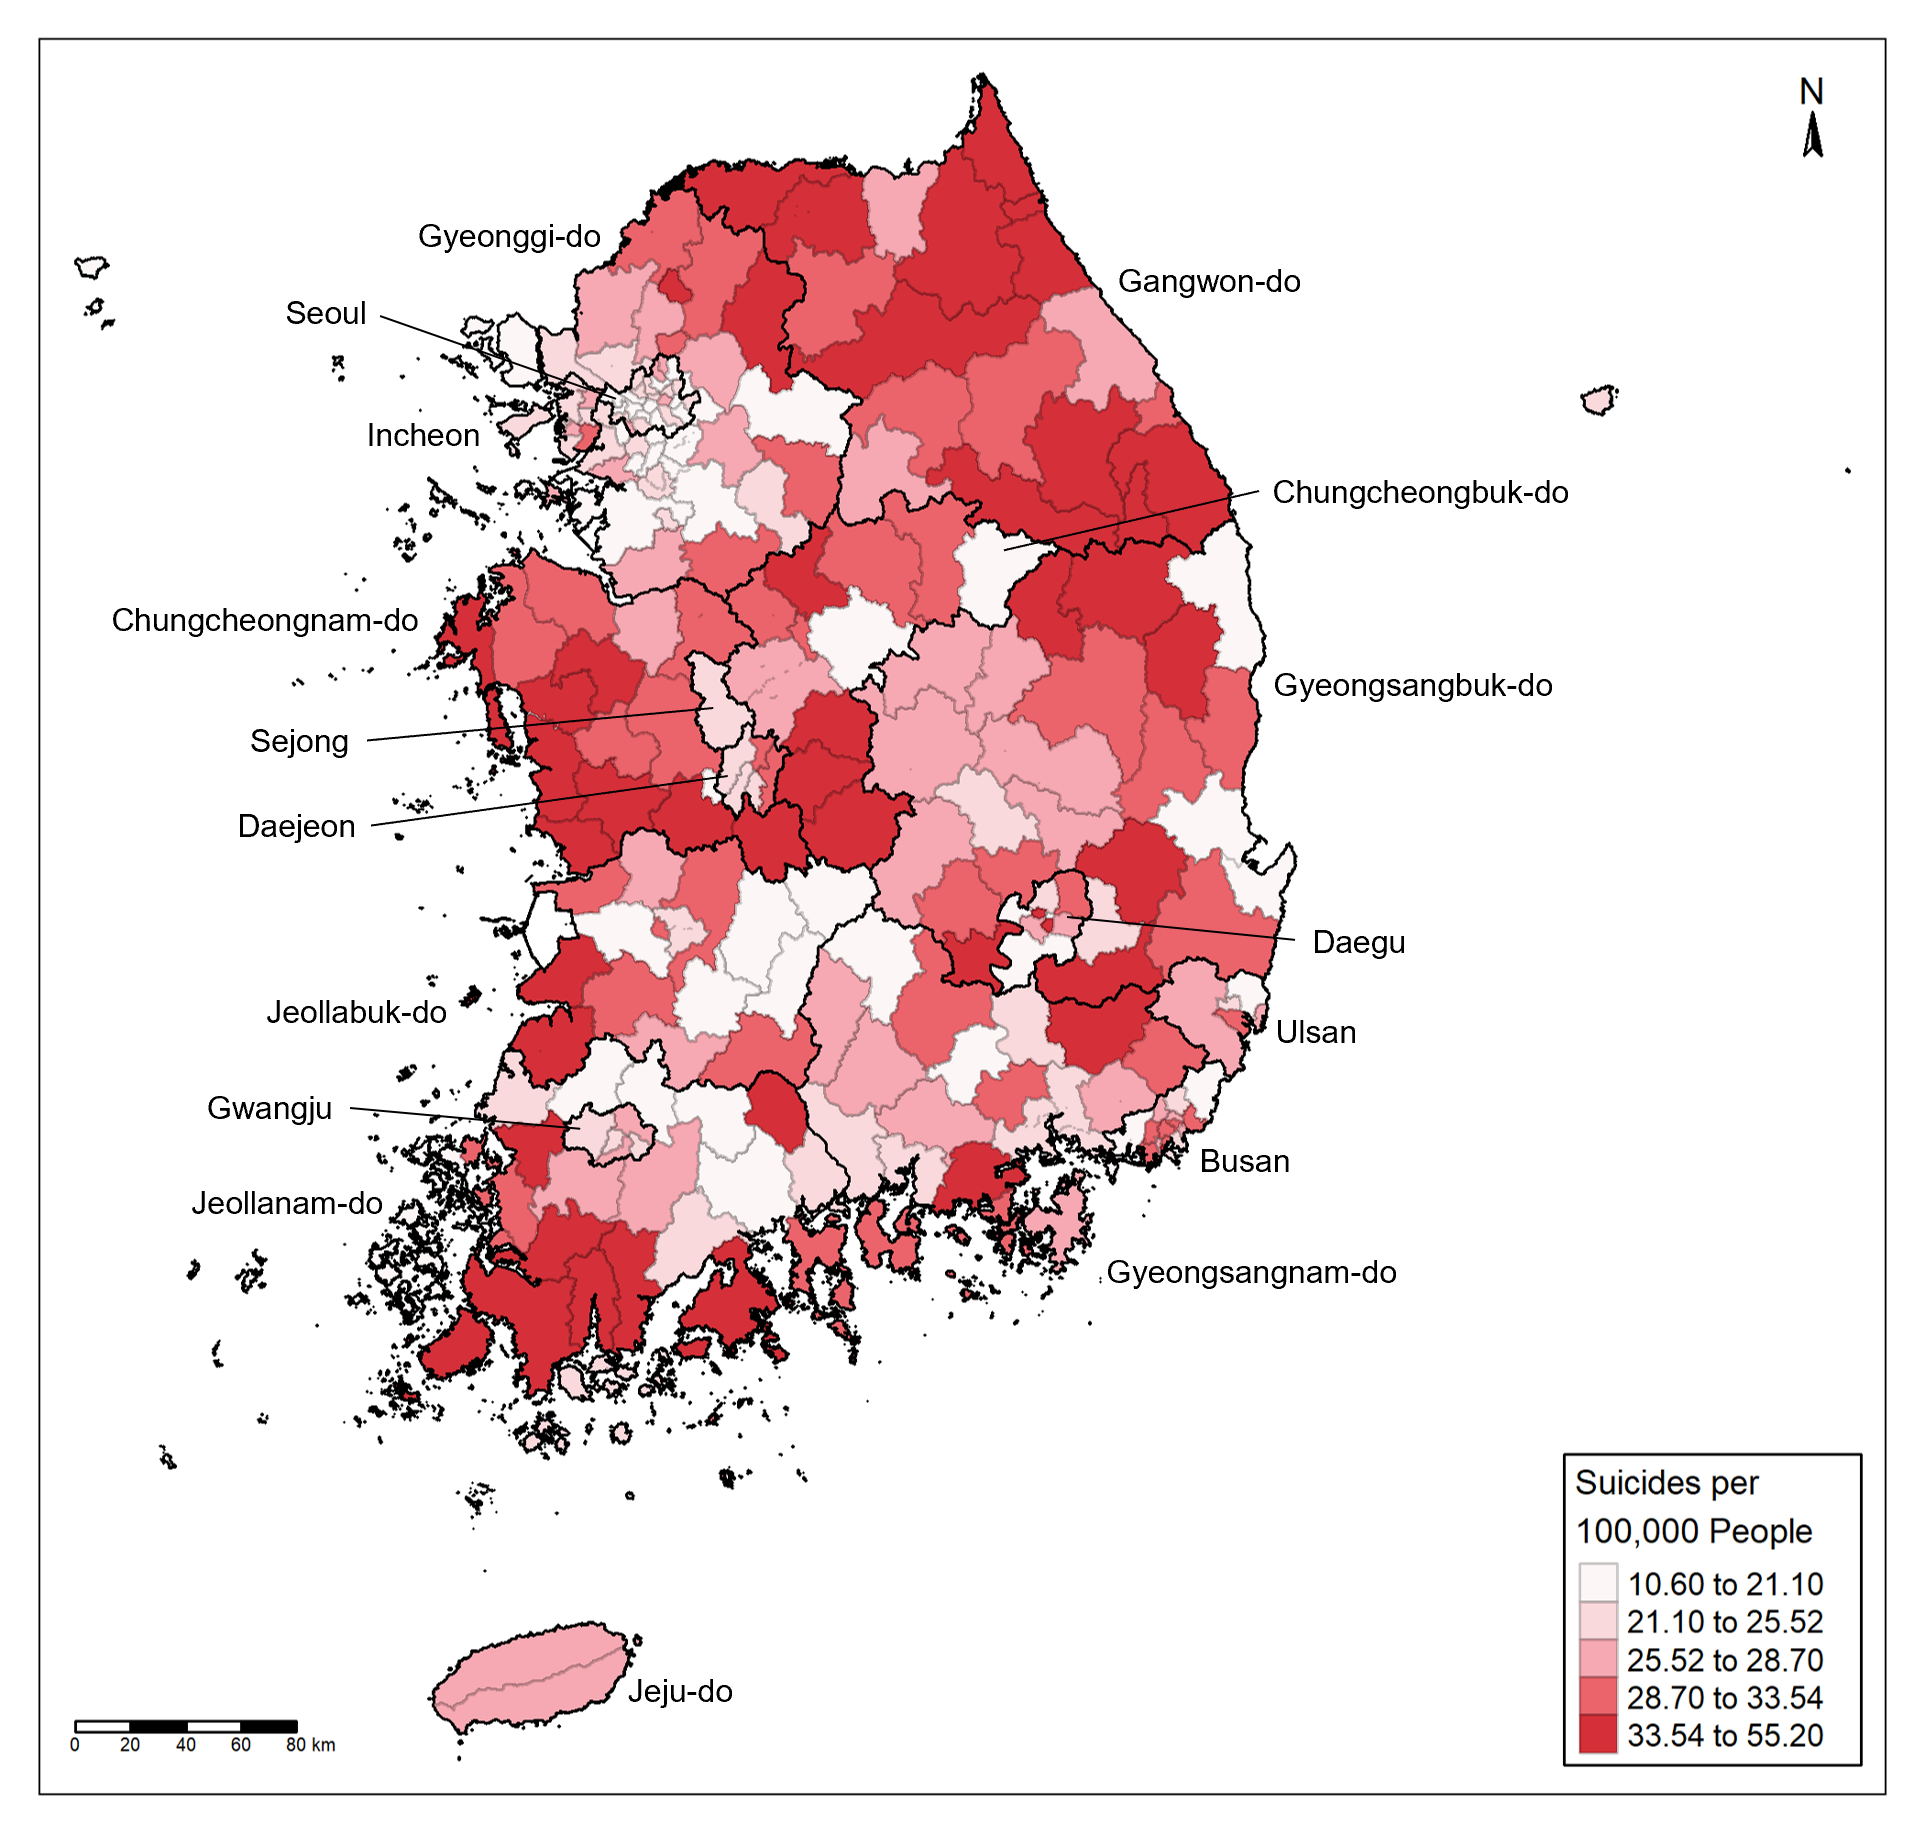
\includegraphics[width=1\textwidth]{assets/suicide_map/suicide_map_2022_annotated.png}
		\label{fig:suicide_map_2022}
	\end{figure}
	
	Suicide rates in 2022 varied significantly across South Korea's 229 municipalities. Higher rates were generally observed in rural and less urbanised areas, particularly in part of Gangwon-do, Chungcheongnam-do, Jeollanam-do, and Gyeongsangbuk-do, where several municipalities recorded over 40 suicides per 100,000 people. In contrast, urban centres such as Seoul and parts of Gyeonggi-do reported markedly lower rates, often below 25. The spatial clustering of high-rate areas suggests regional disparities in factors like healthcare access, economic opportunity, and social support. Most municipalities reported rates well above the OECD average of 11.
	
	\newpage
	\subsection*{1.3 Model Specification}
	
	We employed a Bayesian Poisson regression model with spatial effects to estimate relative risk (RR) of suicide mortality across South Korea's 229 municipalities. To account for spatial autocorrelation between neighbouring areas, we incorporated a structured spatial random effect modelled using an intrinsic conditional autoregressive (ICAR) prior (Besag et al., 1991), a widely used approach in spatial epidemiology. An unstructured random effect was also included to capture residual heterogeneity not explained by spatial structure or covariates.
	
	The model assumes a Poisson likelihood with a log link and a population-based offset, appropriate for modelling rare event counts such as suicide deaths, in small-area epidemiological studies. Spatial adjacency was defined using Queen contiguity, where municipalities sharing either a boundary or vertex were considered neighbours.

	\begin{equation}
		Y_i \sim \text{Poisson}(\lambda_i), \quad 
		\log(\lambda_i) = \log(E_i) + \alpha + \mathbf{X}_i \boldsymbol{\beta} + \sigma \cdot \phi_i\footnote{In the full model, we include both structured and unstructured random effects: 
			$\log(\lambda_i) = \log(E_i) + \alpha + \mathbf{X}_i \boldsymbol{\beta} + \sigma \cdot \left( \sqrt{1 - \rho} \, \theta_i + \sqrt{\rho} \, \phi_i \right)$, where $\theta_i \sim \mathcal{N}(0,1)$ captures unstructured heterogeneity and $\phi_i$ follows an ICAR prior for spatial structure.}
	\end{equation}
	
	Where $Y_i$ denotes the observed number of suicide deaths, $E_i$ the expected count based on population size, $\alpha$ the intercept, $\mathbf{X}_i$ the vector of covariates for municipality $i$, $\boldsymbol{\beta}$ the corresponding coefficients, and $\phi_i$ the spatial random effect scaled by $\sigma$. Structured ($\phi_i$) and unstructured ($\theta_i$) effects are combined through a weighted average governed by $\rho$.
	
	We specified the following priors:
	
	\vspace{1em}
	
	\begin{itemize}
		\item $\alpha \sim \mathcal{N}(0, 1)$ \hfill \textit{(intercept)}
		\item $\boldsymbol{\beta} \sim \mathcal{N}(0, 1)$ \hfill \textit{(covariate coefficients)}
		\item $\theta_i \sim \mathcal{N}(0, 1)$ \hfill \textit{(unstructured random effects)}
		\item $\phi \sim \text{ICAR}(N, \texttt{node1}, \texttt{node2})$ \hfill \textit{(structured spatial random effects)}
		\item $\textstyle \sum_{i=1}^N \phi_i \sim \mathcal{N}(0, 0.001 \cdot N)$ \hfill \textit{(sum-to-zero constraint on $\phi$ to ensure identifiability)}
		\item $\sigma \sim \mathcal{N}(0, 1)$ \hfill \textit{(scaling factor for spatial effects)}
		\item $\rho \sim \text{Beta}(0.5, 0.5)$ \hfill \textit{(mixing proportion between structured and unstructured effects)}
	\end{itemize}
	
	\vspace{1em}
	
	All priors were weakly informative, centred around zero to regularise estimates while allowing flexibility to reflect uncertainty without dominating the posterior.
	
	Model fitting was performed in \textit{Stan} using the \textit{rstan} interface in R. We ran six parallel chains with 20,000 iterations each (10,000 warm-up), using the No-U-Turn Sampler (NUTS) with a maximum tree depth of 12. Convergence diagnostics showed good mixing across all parameters with $\hat{R} < 1.05$.
	
	\newpage
	\section*{2. Results and Discussion}
	
	\subsection*{2.1 Global Parameter Estimates}
	
	The model converged successfully with all $\hat{R}$ values below 1.05 and large effective sample sizes ($n_{\text{eff}}$), indicating stable posterior estimates. Posterior summaries for all global parameters are presented in Table~\ref{tab:icar_results}. 
	
	\begin{table}[H]
		\centering
		\caption{Posterior Estimates of Global Parameters}
		\renewcommand{\arraystretch}{1.3}
		\begin{tabular}{cccccccc}
			\hline
			\textbf{Parameter} & \textbf{Mean} & \textbf{SE Mean} & \textbf{2.5\% CrI} & \textbf{97.5\% CrI} & \boldmath{$n_\text{eff}$} & \boldmath{$\hat{R}$} \\
			\hline
			$\alpha$   & $-0.1956$ & $0.0008$ & $-0.4548$ & $0.0685$ & $25689.1$ & $1.0005$ \\
			$\beta_1$  & $0.0120$  & $0.0000$ & $0.0067$  & $0.0174$ & $27152.2$ & $1.0003$ \\
			$\beta_2$  & $-0.0052$ & $0.0000$ & $-0.0139$ & $0.0035$ & $26780.3$ & $1.0001$ \\
			$\beta_3$  & $-0.0385$ & $0.0002$ & $-0.0706$ & $-0.0065$ & $9776.5$  & $1.0007$ \\
			$\beta_4$  & $0.0089$  & $0.0000$ & $-0.0014$ & $0.0190$ & $28092.1$ & $1.0001$ \\
			$\sigma$   & $0.2118$  & $0.0003$ & $0.1611$  & $0.2685$ & $7507.3$  & $1.0006$ \\
			\hline
		\end{tabular}
		
		\vspace{0.5em}
		
		\begin{minipage}{0.9\textwidth}
			\vspace{0.5em}
			\footnotesize
			\textit{Note.} SE Mean = Standard Error of Posterior Mean; CrI = Credible Interval; $n_\text{eff}$ indicates the effective sample size. $\hat{R}$ is the Gelman–Rubin convergence diagnostic, where values near 1.00 suggest good convergence.
		\end{minipage}
		\label{tab:icar_results}
	\end{table}
	
	The global intercept ($\alpha$) was estimated at $-0.20$, corresponding to a relative risk (RR) of $\exp(-0.20) \approx 0.82$ (95\% CrI: 0.63 to 1.07). This suggests a slightly lower-than-expected baseline suicide risk across municipalities, though the result is not statistically significant as the credible interval includes the null value of 1.00.
	
	Among the covariates, the unemployment rate ($\beta_3$) showed the strongest association with suicide risk. with a one-unit increase in unemployment associated with a 4\% decrease in relative risk (RR ≈ 0.96; 95\% CrI: 0.93 to 0.99). The upper bound narrowly excludes 1.00, suggesting a potentially meaningful but counter-intuitive negative effect.
	
	Both the single-person household ratio ($\beta_1$) and unmet medical needs rate ($\beta_4$) were associated with modest increases in suicide risk (RRs ≈ 1.01). However their credible intervals either narrowly include or approach the null value, indicating weak positive effects. The stress awareness rate showed a slight negative association (RR = 0.99; 95\% CrI: 0.99 to 1.00), though the effect was marginal.
	
	The spatial standard deviation $\sigma$ was estimated at 0.21 (95\% CrI: 0.16 to 0.27), indicating moderate residual spatial variation in suicide risk. This supports the inclusion of spatially structured random effects in the model.

	\subsection*{2.2 Spatial Distribution of Relative Risk}

	\begin{figure}[H]
		\centering
		\caption{Relative Risk Across South Korean Municipalities}
		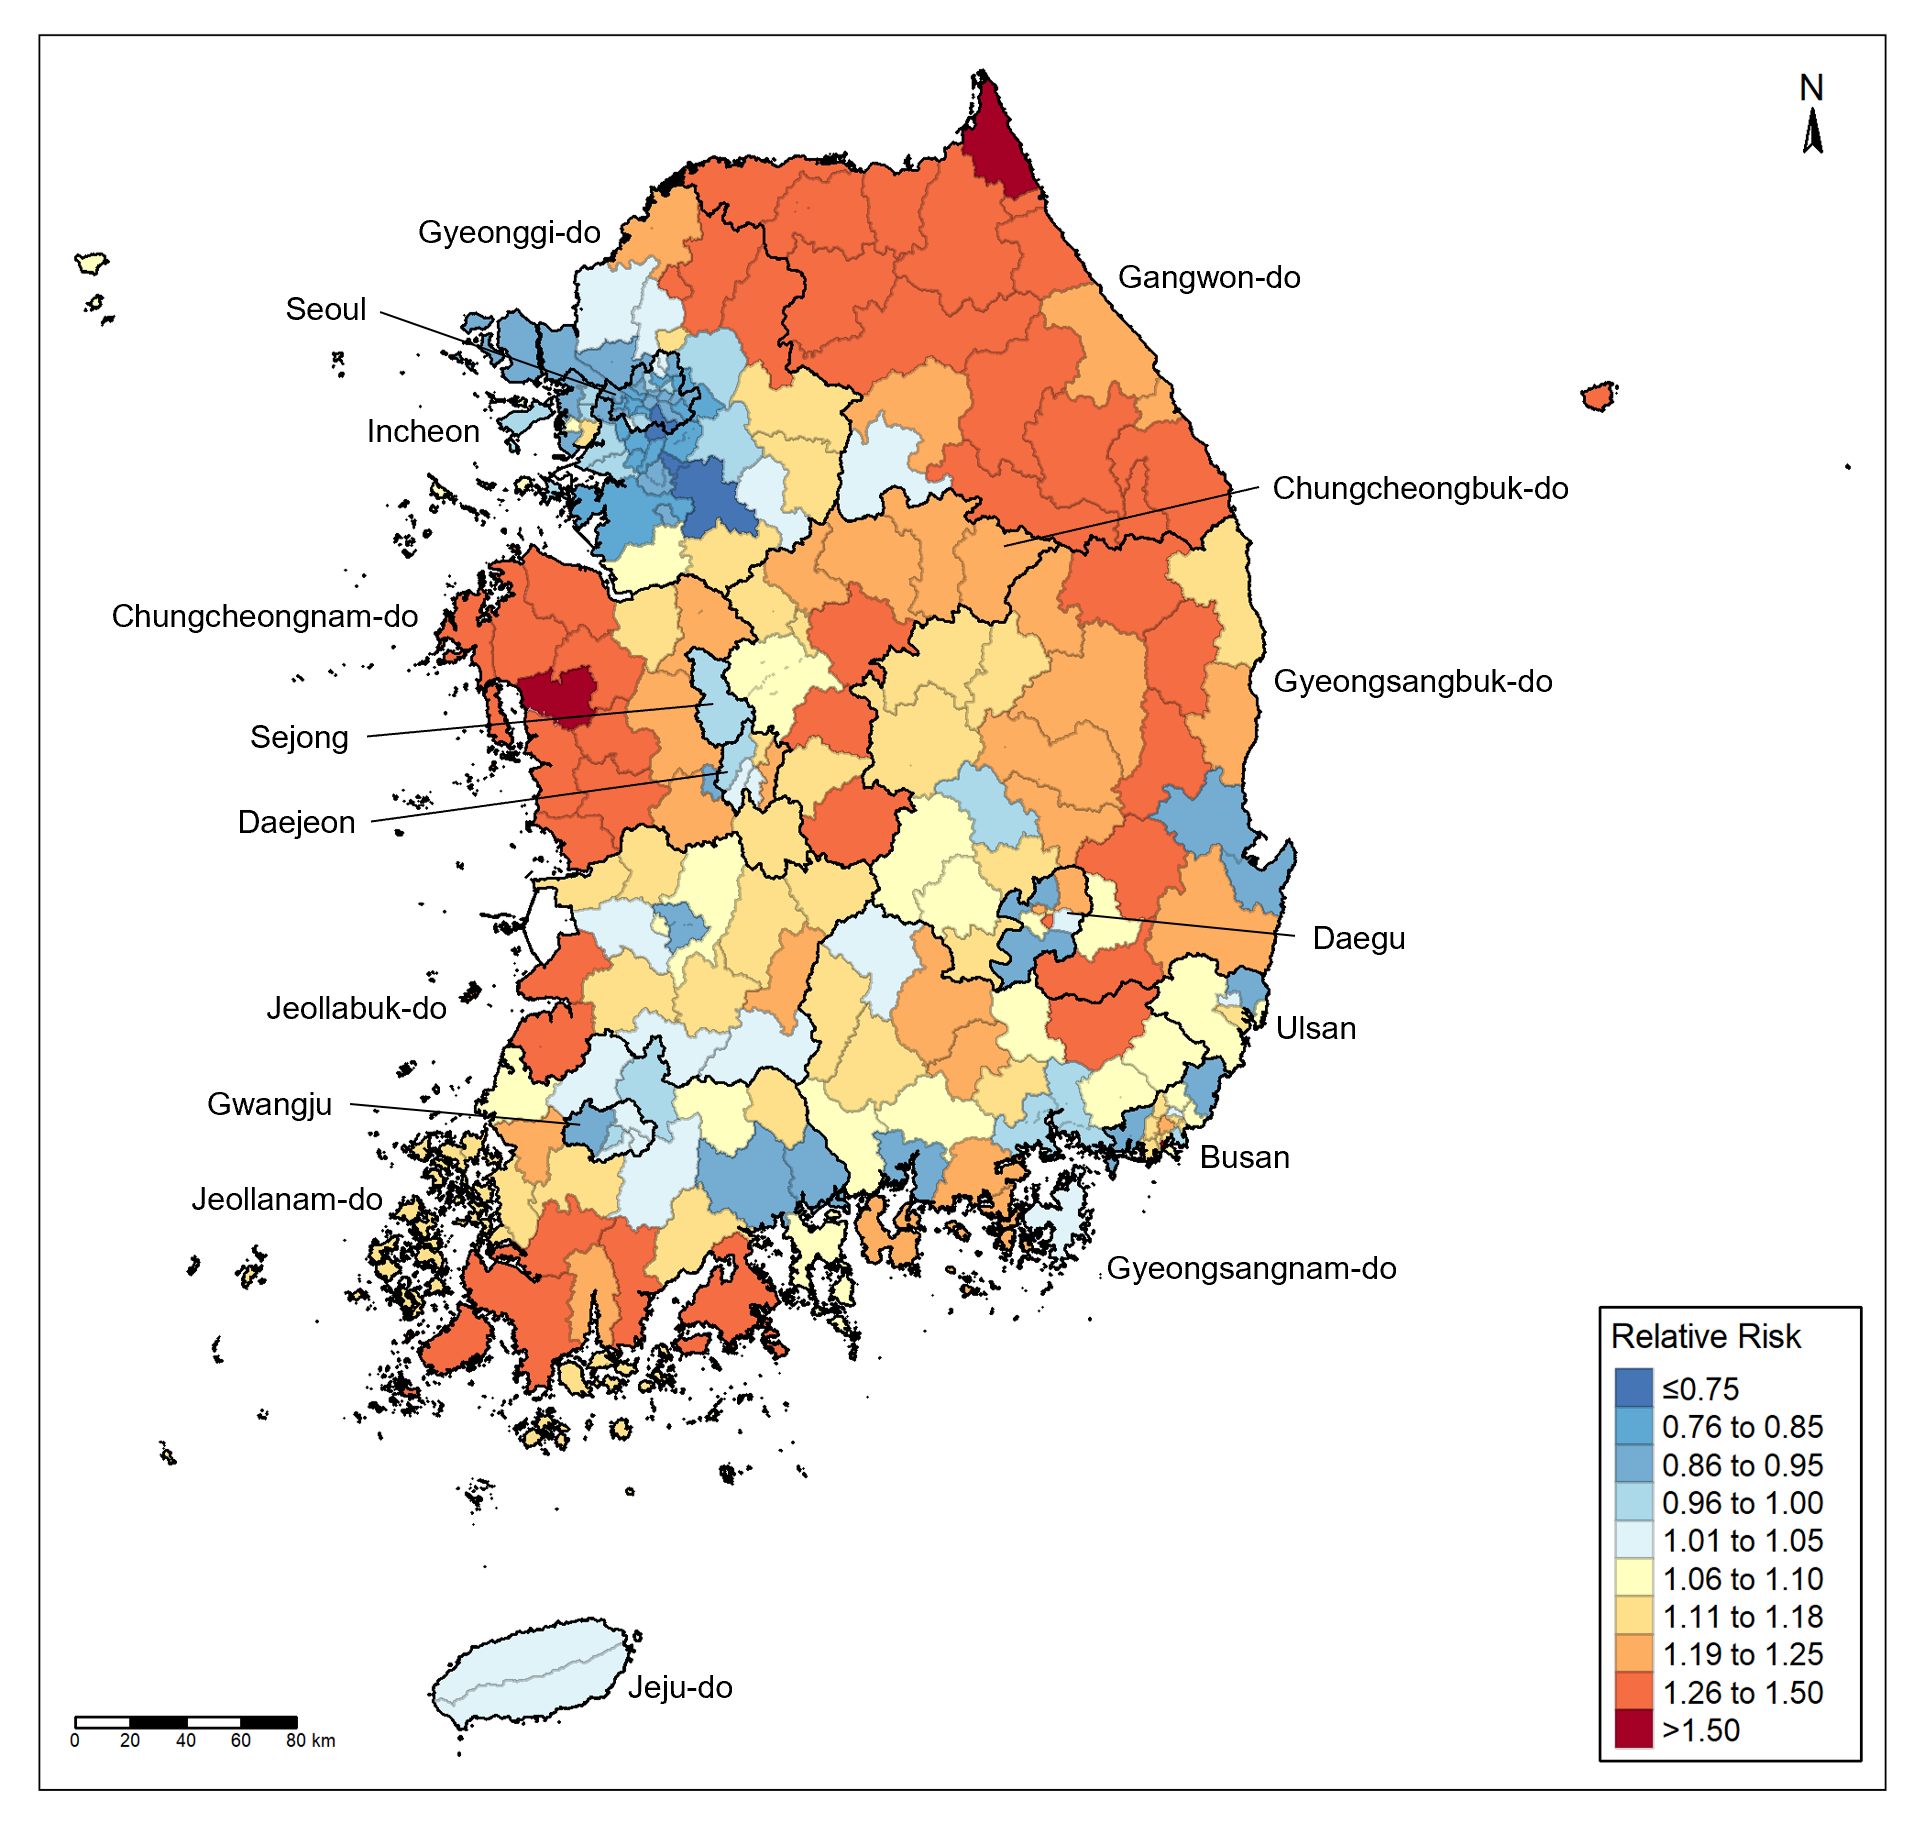
\includegraphics[width=1\textwidth]{assets/relative_risk/relative_risk_map_2022_annotated.png}
		\label{fig:relative_risk_map}
	\end{figure}

	Figure~\ref{fig:relative_risk_map} reveals markedspatial disparities in the relative risk (RR) of suicide mortality across South Korean municipalities. High-risk areas (RR > 1.25) are prominently clustered in rural areas, particularly in Chungcheongnam-do, Chungcheongbuk-do, Gangwon-do and Gyeongsangbuk-do. Municipalities such as Hongseong-gun in Chungcheongnam-do and Goseong-gun in Gangwon-do exceeds an RR of 1.50—the highest observed category. These areas are largely peripheral and rural, often characterised by again ppoulations, limited access to mental health services, economic vulnerability, and weaker social networks. Rural municipalities also tend to feature a higher proportion of older and male populations—both typically associated with elevated suicide risk.
	
	In contrast, most low-risk clusters (RR < 1.00) are concentrated in urbanised centres, especially within the Seoul Metropolitan Area encompassing Seoul, Incheon and Gyeonggi-do. Other metropolitan cities such as Busan, Daegu and Gwangju also exhibit lower-than-expected suicide risk after adjusting for covariates. These urban regions may benefit from denser healthcare infrastructure, better economic prospects, and stronger social integration. The spatial clustering of high and low RR values indicates substantial spatial autocorrelation and reinforces the rationale  for including of spatial random effects in the model. Overall, the results demonstrate a pronounced urban-rural divide in suicide risk, as well as disparities between the capital region and the rest of the country.

	\subsection*{2.3 Statistical Significance of Relative Risk}
	
	\begin{figure}[H]
		\centering
		\caption{Statistical Significance of Relative Risk Across South Korean Municipalities}
		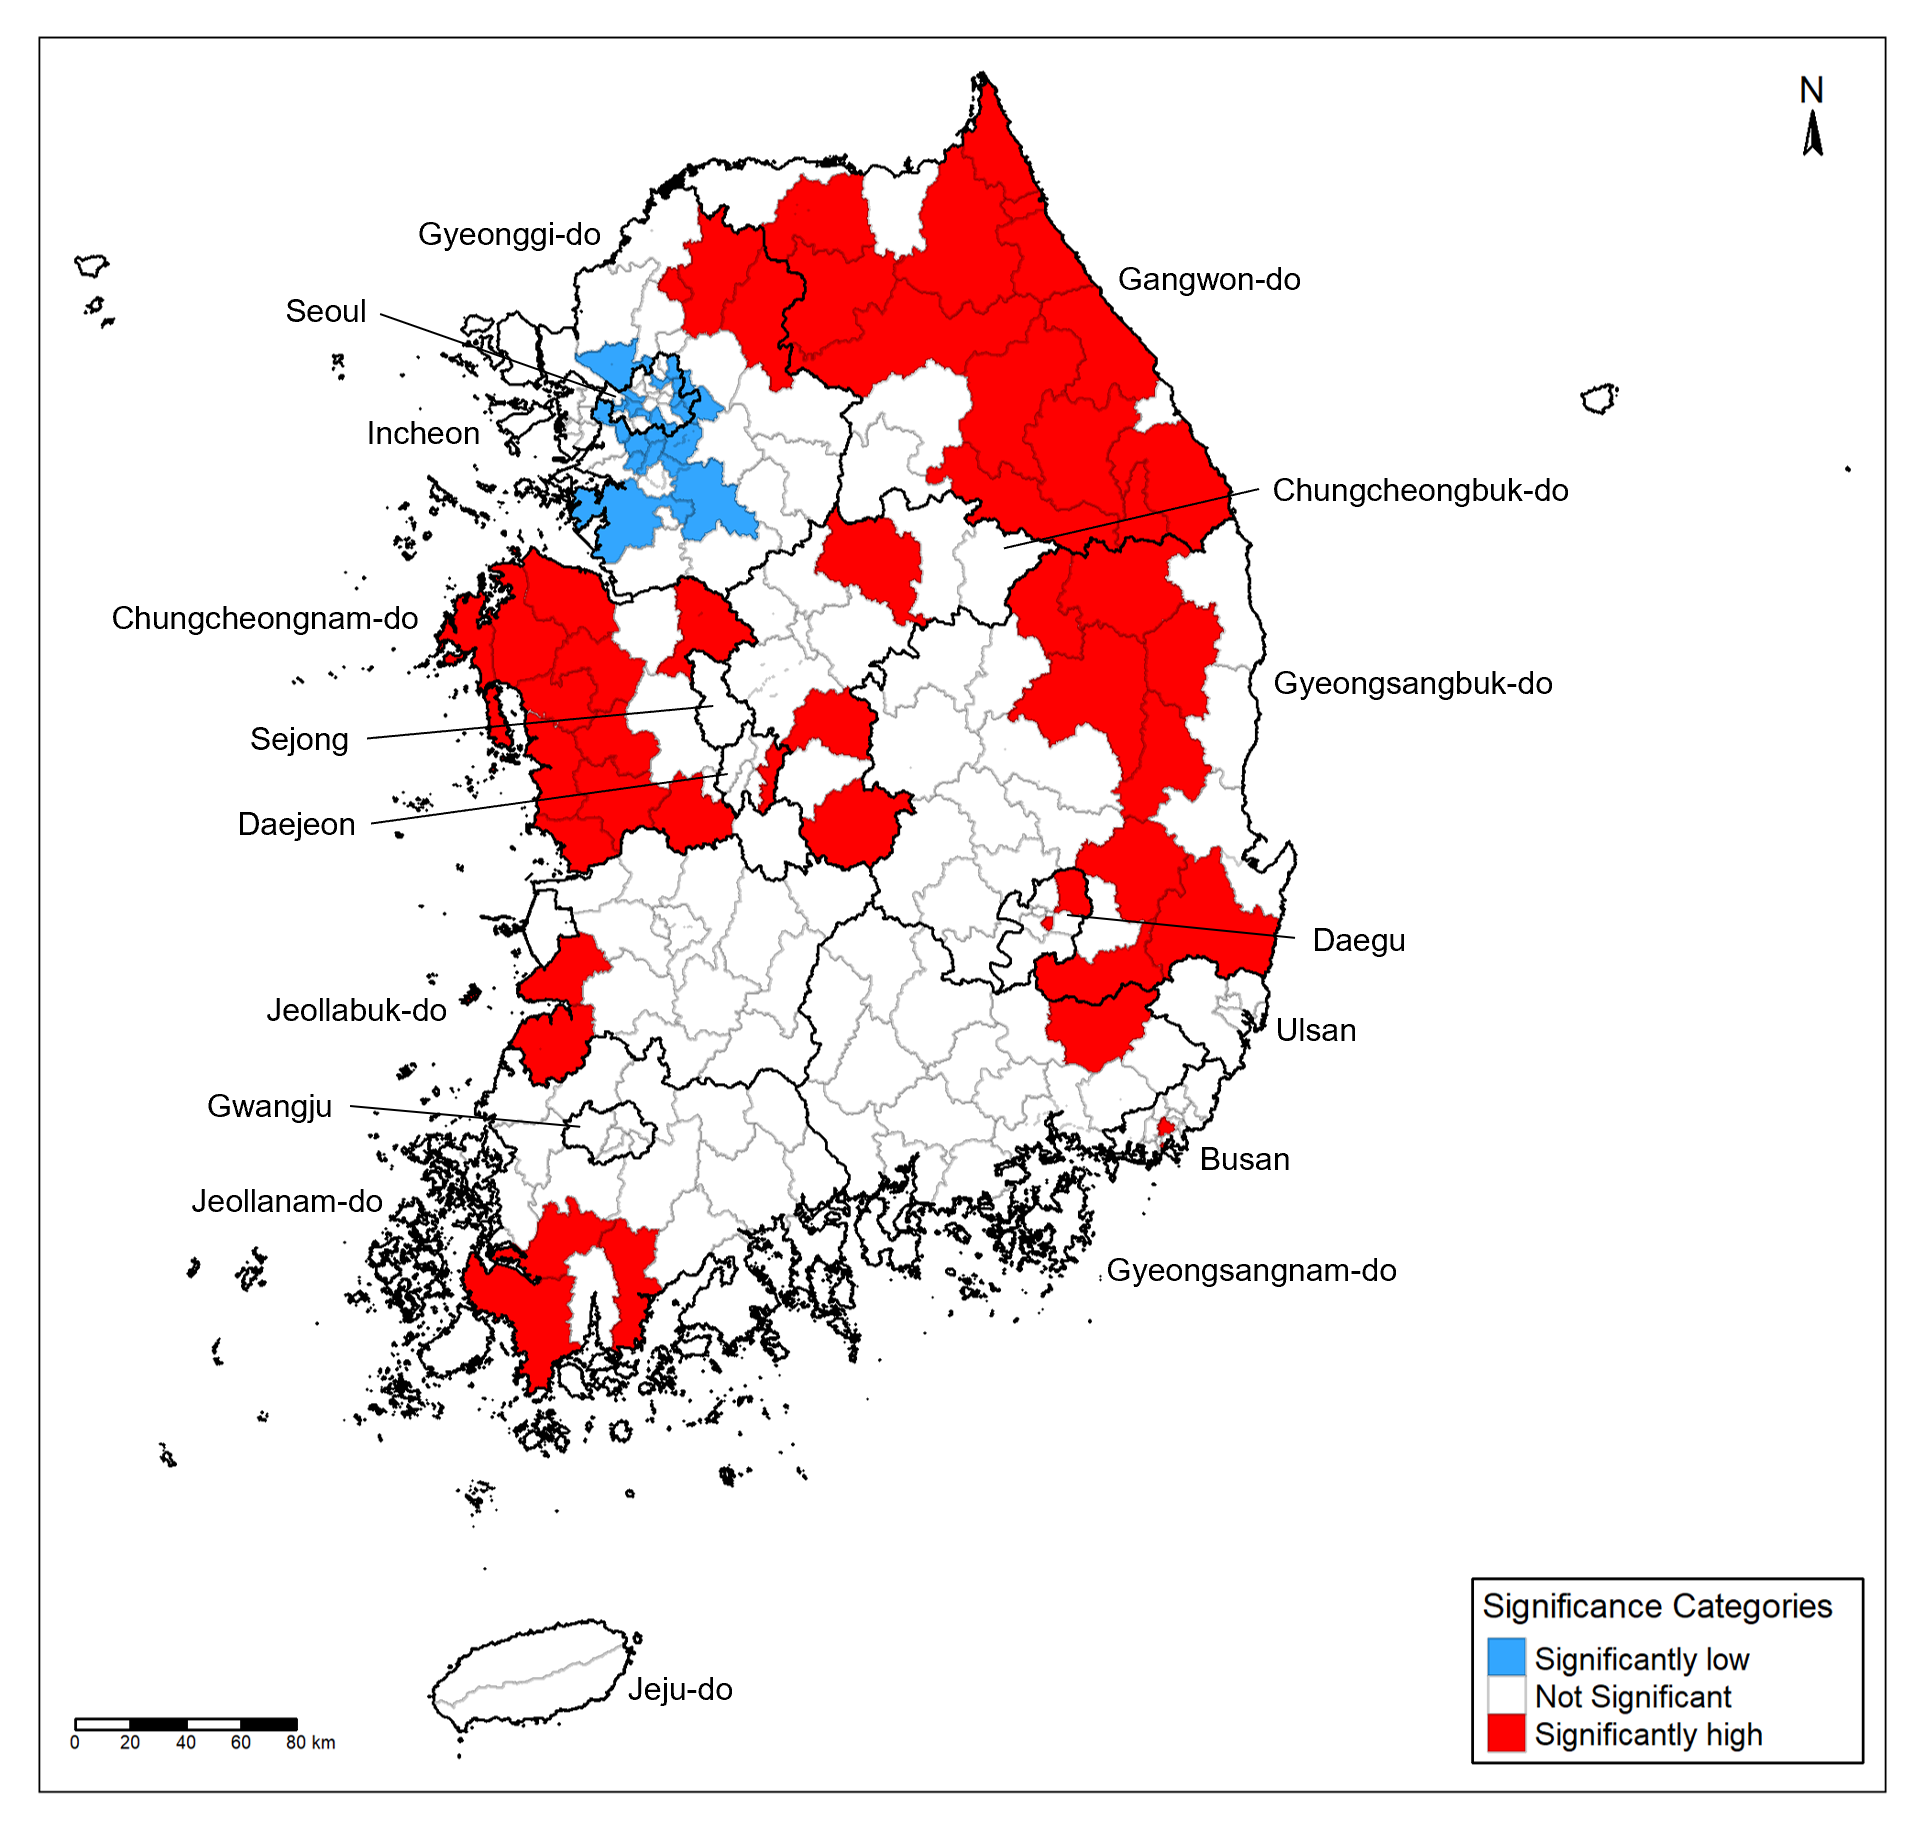
\includegraphics[width=1\textwidth]{assets/significance_categories/significance_categories_map_2022_annotated.png}
		\label{fig:significance_map}
	\end{figure}

	Figure~\ref{fig:significance_map} presents the statistical significance of relative risk estimates. Municipalities shaded in red indicate significantly elevated suicide risk, where the entire 95\% credible interval lies above 1.00. These areas are concentrated in rural regions, particularly in Gangwon-do, Chungcheongnam-do, Gyeongsangbuk-do, and parts of Jeollanam-do, reinforcing earlier findings.
	
	In contrast, blue areas denote municipalities with significantly lower-than-expected suicide risk. with 95\% CrI entirely below 1.00. The only low-risk cluster appears in the Seoul Metropolitan Area (Seoul, Incheon, and Gyeonggi-do), highlighting the potential protective effects of urban infrastructure, access to services, and economic opportunity. The majority of municipalities, shown in white, have non-significant risk levels.
	
	\subsection*{2.4 Exceedance Probabilities}
	
	\begin{figure}[H]
		\centering
		\caption{Exceedance Probabilities Across South Korean Municipalities}
		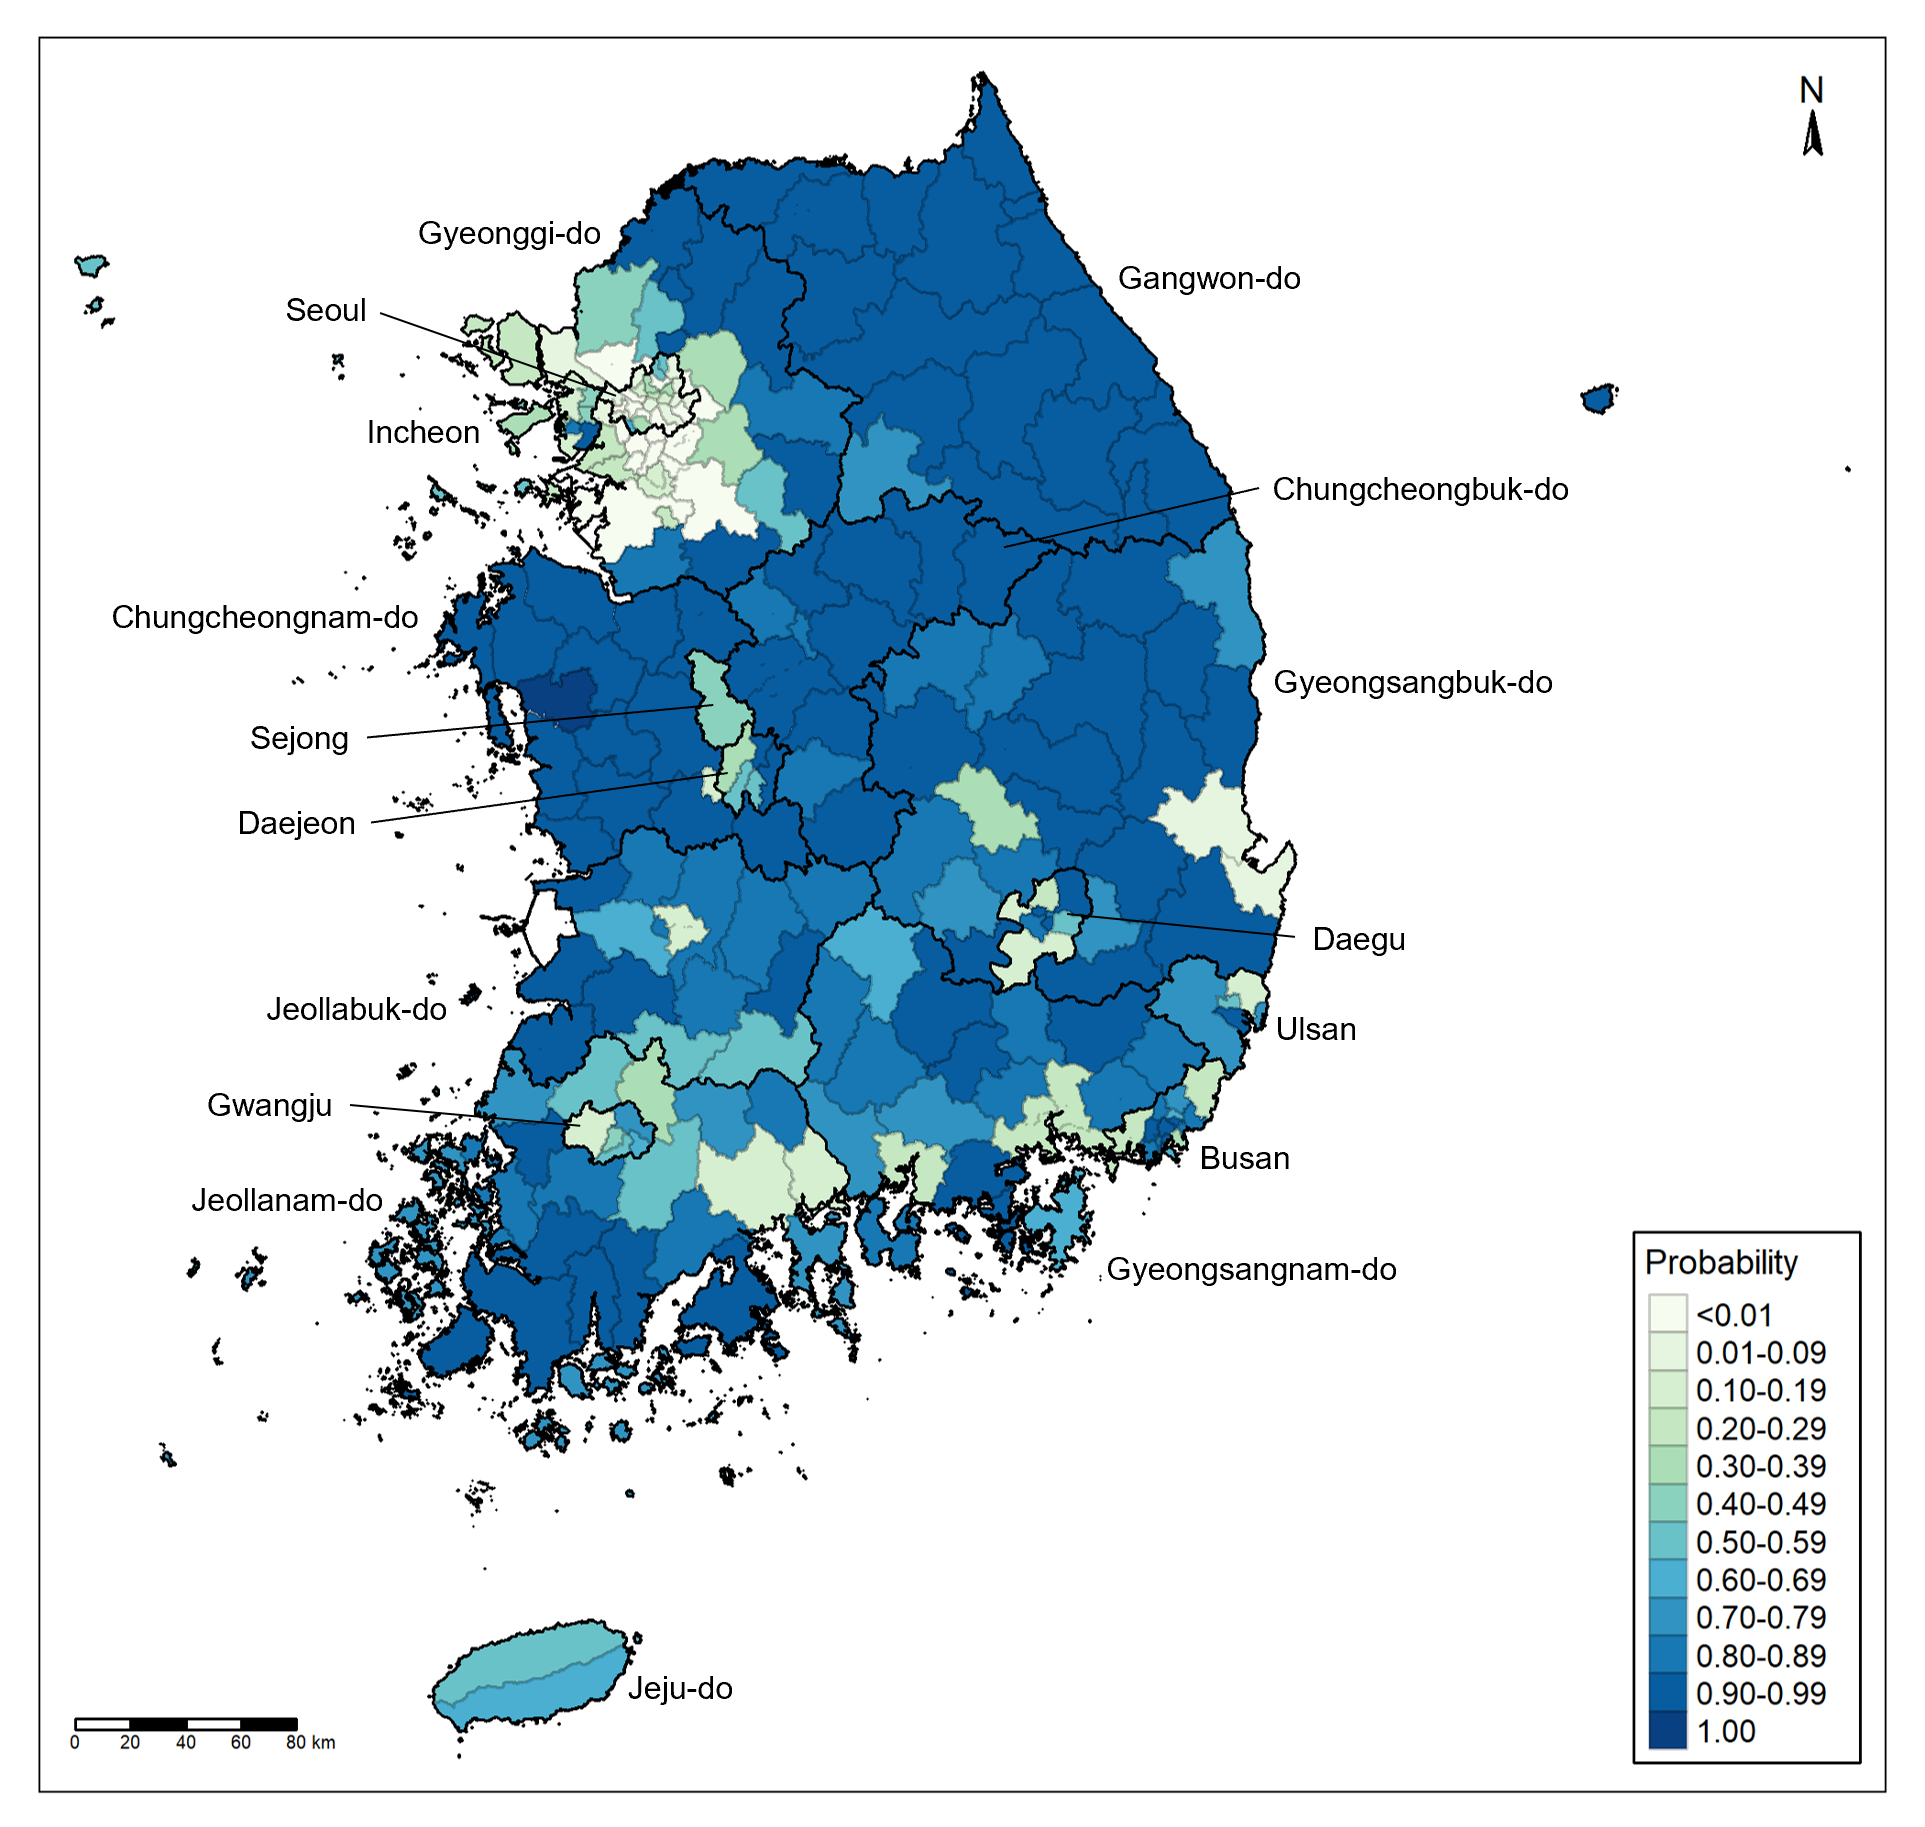
\includegraphics[width=1\textwidth]{assets/exceedance_probabilities/exceedance_probabilities_map_2022_annotated.png}
		\label{fig:exceedance_probabilities_map}
	\end{figure}
	
	Figure~\ref{fig:exceedance_probabilities_map} shows the posterior probability that each municipality's relative risk (RR) of suicide exceeds 1.00. Darker blue municipalities exhibit high exceedance probabilities (≥0.90), indicating strong posterior evidence of elevated suicide risk. These high-probability areas are widespread across non-capital regions. In contrast, the Seoul Metropolitan Area shows consistently low exceedance probabilities, forming a stark visual contrast. This pronounced divide between capital and non-capital regions highlights the spatial inequities in suicide risk and calls for policymakers to look beyond the capital for targeted mental health interventions.

	\subsection*{2.5 Discussion}
	
	The results carry important policy implications. Most notably, the unemployment rate showed the strongest association with suicide risk, with a one-unit increase linked to a 4\% decrease in relative risk. Though counter-intuitive, this may reflect the buffering effect of South Korea's unemployment benefits, which allow individuals to maintain economic stability while avoiding chronic workplace stressors such as long hours, intense competition, and rigid hierarchies. While strong safety nets can offer psychological protection, they may also incentivise withdrawal from the highly stressful labour market, raising concerns about economic inactivity and long-term fiscal strain. These findings suggest that improving workplace mental health should be a priority, rather than relying solely on income support systems.
	
	Single-person household ratio and unmet medical needs rate show weak but positive associations with suicide risk, highlighting the relevance of social connection and access to healthcare. These findings align with existing literature and support continued investment in community formation, outreach to isolated individuals, and expansion of affordable mental health services.
	
	Geographically, a sharp divide emerges between the Seoul Metropolitan Area and the rest of the country. Rural municipalities exhibit consistently higher relative risk and exceedance probabilities, while Seoul, Incheon, and Gyeonggi-do appear comparatively insulated. This suggests that national strategies risk neglecting the distinct vulnerabilities of peripheral regions, especially when policymakers themselves are based in the capital region. To address these disparities, policymakers should prioritise decentralised mental health services, enhance tele-health and transportation infrastructure, and pursue regional development strategies that foster economic opportunity and social cohesion outside the capital.
	
	Nonetheless, this study has several limitations. Although preliminary diagnostics indicated modest overdispersion in suicide counts ($\theta \approx 1.28$), we opted for a Poisson model due to its interpretability and established use in spatial epidemiology. The manual linking of disconnected subgraphs using centroid proximity ensured spatial contiguity but may not reflect true socioeconomic similarity, potentially biasing results in island geographies. The analysis is also cross-sectional, relying solely on 2022 data, and thus cannot capture temporal dynamics. Finally, the counter-intuitive finding that higher unemployment is associated with lower suicide risk could be confounded by unmeasured factors such as informal employment or labour market inactivity, where only those actively seeking employment are classified as unemployed.
	
	\subsection*{2.6 Conclusion}
	
	Despite these limitations, the study offers valuable insights into the spatial dynamics of suicide risk in South Korea. By combining small-area estimation with literature-informed covariates, it highlights the urgent need for geographically differentiated suicide prevention strategies that extend beyond the capital region and call for counter-intuitive thinking in policy design.
	
%	\section*{References}
%	
%	\begin{flushleft}
%		\begin{thebibliography}{9}
%			\bibitem{WHO2023}
%			World Health Organization. (2023). \textit{Suicide Worldwide in 2022: Global Health Estimates}. Geneva: WHO.
%			
%			\bibitem{Rue2005}
%			Rue, H., Martino, S., & Chopin, N. (2009). \textit{Approximate Bayesian inference for latent Gaussian models using integrated nested Laplace approximations (INLA)}. Journal of the Royal Statistical Society, Series B, 71(2), 319--392.
%			
%			\bibitem{Lee2011}
%			Lee, D. (2011). \textit{A comparison of conditional autoregressive models used in Bayesian disease mapping}. Spatial and Spatio-temporal Epidemiology, 2(2), 79--89.
%			
%			\bibitem{Zhu2006}
%			Zhu, L., Gorman, D. M., & Horel, S. (2006). \textit{Hierarchical Bayesian spatial models for alcohol availability, drug "hot spots," and violent crime}. International Journal of Health Geographics, 5(1), 54.
%			
%			\bibitem{StatisticsKorea2022}
%			Statistics Korea. (2023). \textit{Population and Health Indicators by Municipality}. Daejeon: KOSIS.
%		\end{thebibliography}
%	\end{flushleft}

%Kim, E. and Kim, S. (2024). Spatially clustered patterns of suicide mortality rates in South Korea: a geographically weighted regression analysis. BMC Public Health, 24(1). doi:https://doi.org/10.1186/s12889-024-19899-4.
	
\end{document}

